\documentclass{CInf_practice}

% Avoid waiting for all the foreach loops
\newcounter{QUICK}
\setcounter{QUICK}{1}

\sheet{5}{Programmierbare Bausteine, Hazards und Flipflops}
\begin{document}
\cinftitle

\ex{Bit-Slice-ALU}{6 + 8 + 16 + 4 = 34}
\subex{}
\begin{center}
   \begin{tabular}{cc|ccc||cc}
      $s_1$ & $s_0$ & $a_i$ & $b_i$ & $c_{i-1}$ & $y_i$ & $c_i$ \\\hline
      0 & 0 & 0 & 0 & 0 & 0 & 0 \\
      0 & 0 & 0 & 0 & 1 & 1 & 0 \\
      0 & 0 & 0 & 1 & 0 & 1 & 0 \\
      0 & 0 & 0 & 1 & 1 & 0 & 1 \\
      0 & 0 & 1 & 0 & 0 & 1 & 0 \\
      0 & 0 & 1 & 0 & 1 & 0 & 1 \\
      0 & 0 & 1 & 1 & 0 & 0 & 1 \\
      0 & 0 & 1 & 1 & 1 & 1 & 1 \\
      0 & 1 & 0 & 0 & 0 & 0 & 0 \\
      0 & 1 & 0 & 0 & 1 & 1 & 1 \\
      0 & 1 & 0 & 1 & 0 & 1 & 1 \\
      0 & 1 & 0 & 1 & 1 & 0 & 1 \\
      0 & 1 & 1 & 0 & 0 & 1 & 0 \\
      0 & 1 & 1 & 0 & 1 & 0 & 0 \\
      0 & 1 & 1 & 1 & 0 & 0 & 0 \\
      0 & 1 & 1 & 1 & 1 & 1 & 1 \\
      1 & 0 & 0 & 0 & 0 & 0 & X \\
      1 & 0 & 0 & 0 & 1 & 0 & X \\
      1 & 0 & 0 & 1 & 0 & 0 & X \\
      1 & 0 & 0 & 1 & 1 & 0 & X \\
      1 & 0 & 1 & 0 & 0 & 0 & X \\
      1 & 0 & 1 & 0 & 1 & 0 & X \\
      1 & 0 & 1 & 1 & 0 & 1 & X \\
      1 & 0 & 1 & 1 & 1 & 1 & X \\
      1 & 1 & 0 & 0 & 0 & 1 & X \\
      1 & 1 & 0 & 0 & 1 & 1 & X \\
      1 & 1 & 0 & 1 & 0 & 1 & X \\
      1 & 1 & 0 & 1 & 1 & 1 & X \\
      1 & 1 & 1 & 0 & 0 & 0 & X \\
      1 & 1 & 1 & 0 & 1 & 0 & X \\
      1 & 1 & 1 & 1 & 0 & 0 & X \\
      1 & 1 & 1 & 1 & 1 & 0 & X 
   \end{tabular}
\end{center}

\subex{}
$y_i$:
\begin{center}
   \begin{tikzpicture}
      \matrix (m)[
         nodes={matrix node},
         matrix of nodes,
         inner sep=0pt,
         outer sep=0pt,
         row sep=-.5pt,
         column sep=-.5pt
      ]  {
         0 & 1 & 0 & 1 & 0 & 0 & 0 & 0 \\
         1 & 0 & 1 & 0 & 1 & 1 & 0 & 0 \\
         1 & 0 & 1 & 0 & 0 & 0 & 1 & 1 \\
         0 & 1 & 0 & 1 & 0 & 0 & 1 & 1 \\
      };

      
      \draw[|-|] ($(m-1-5.north west) + (0,2.2cm)$) -- node[above] () {$s_1$} ($(m-1-8.north east) + (0,2.2cm)$);
      \draw[|-|] ($(m-1-3.north west) + (0,1.4cm)$) -- node[above] () {$a_i$} ($(m-1-6.north east) + (0,+1.4cm)$);
      \draw[|-|] ($(m-1-2.north west) + (0,.6cm)$) -- node[above] () {$c_{i-1}$} ($(m-1-3.north east) + (0,0.6cm)$);
      \draw[|-|] ($(m-1-6.north west) + (0,.6cm)$) -- node[above] () {$c_{i-1}$} ($(m-1-7.north east) + (0,0.6cm)$);
      \draw[|-|] ($(m-2-1.north west) + (-.6cm,0)$) -- node[left] () {$b_i$} ($(m-3-1.south west) + (-.6cm,0)$);
      \draw[|-|] ($(m-3-1.north west) + (-1.2cm,0)$) -- node[left] () {$s_0$} ($(m-4-1.south west) + (-1.2cm,0)$);

      \clip ($(m.north west) + (-8pt,8pt)$) rectangle ($(m.south east) + (8pt,-8pt)$);
      \draw[highlight,draw=red] ($(m-2-1.north west) + (3pt,-3pt)$) rectangle ($(m-3-1.south east) + (-3pt,3pt)$);
      \draw[highlight] ($(m-2-3.north west) + (3pt,-3pt)$) rectangle ($(m-3-3.south east) + (-3pt,3pt)$);
      \draw[highlight,draw=olive,dashed] ($(m-4-2.north west) + (3pt,-3pt)$) rectangle ($(m-4-2.south east) + (-3pt,-1cm)$);
      \draw[highlight,draw=olive,dashed] ($(m-1-2.south east) + (-3pt,3pt)$) rectangle ($(m-1-2.north west) + (3pt,1cm)$);
      \draw[highlight,loosely dashed] ($(m-4-4.north west) + (3pt,-3pt)$) rectangle ($(m-4-4.south east) + (-3pt,-1cm)$);
      \draw[highlight,loosely dashed] ($(m-1-4.south east) + (-3pt,3pt)$) rectangle ($(m-1-4.north west) + (3pt,1cm)$);
      \draw[highlight] ($(m-2-5.north west) + (3pt,-3pt)$) rectangle ($(m-2-6.south east) + (-3pt,3pt)$);
      \draw[highlight] ($(m-3-7.north west) + (3pt,-3pt)$) rectangle ($(m-4-8.south east) + (-3pt,3pt)$);
   \end{tikzpicture}
   $y_i = \comp s_1\comp a_i \comp b_i c_{i-1} + \comp s_1 \comp a_i b_i \comp
   c_{i-1} + \comp s_1 a_i \comp b_i \comp c_{i-1} + \comp s_1 a_i b_i c_{i-1} + s_1
   \comp s_0 a_i b_i + s_1 s_0 \comp a_i$
\end{center}

$c_i$:
\begin{center}
   \begin{tikzpicture}
      \matrix (m)[
         nodes={matrix node},
         matrix of nodes,
         inner sep=0pt,
         outer sep=0pt,
         row sep=-.5pt,
         column sep=-.5pt
      ]  {
         0 & 0 & 1 & 0 & X & X & X & X \\
         0 & 1 & 1 & 1 & X & X & X & X \\
         1 & 1 & 1 & 0 & X & X & X & X \\
         0 & 1 & 0 & 0 & X & X & X & X \\
      };

      \draw[|-|] ($(m-1-5.north west) + (0,2.2cm)$) -- node[above] () {$s_1$} ($(m-1-8.north east) + (0,2.2cm)$);
      \draw[|-|] ($(m-1-3.north west) + (0,1.4cm)$) -- node[above] () {$a_i$} ($(m-1-6.north east) + (0,+1.4cm)$);
      \draw[|-|] ($(m-1-2.north west) + (0,.6cm)$) -- node[above] () {$c_{i-1}$} ($(m-1-3.north east) + (0,0.6cm)$);
      \draw[|-|] ($(m-1-6.north west) + (0,.6cm)$) -- node[above] () {$c_{i-1}$} ($(m-1-7.north east) + (0,0.6cm)$);
      \draw[|-|] ($(m-2-1.north west) + (-.6cm,0)$) -- node[left] () {$b_i$} ($(m-3-1.south west) + (-.6cm,0)$);
      \draw[|-|] ($(m-3-1.north west) + (-1.2cm,0)$) -- node[left] () {$s_0$} ($(m-4-1.south west) + (-1.2cm,0)$);

      \clip ($(m.north west) + (-8pt,8pt)$) rectangle ($(m.south east) + (8pt,-8pt)$);
      \draw[highlight,draw=red] ($(m-3-2.north east) + (-3pt,-3pt)$) rectangle ($(m-3-1.south east) + (-3cm,3pt)$);
      \draw[highlight,draw=red] ($(m-3-7.north west) + (3pt,-3pt)$) rectangle ($(m-3-8.south east) + (3cm,3pt)$);
      \draw[highlight,dashed] ($(m-3-2.north west) + (3pt,-3pt)$) rectangle ($(m-4-2.south east) + (-3pt,3pt)$);
      \draw[highlight,dashed] ($(m-3-7.north west) + (3pt,-3pt)$) rectangle ($(m-4-7.south east) + (-3pt,3pt)$);
      \draw[highlight,draw=blue,dash dot] ($(m-2-2.north west) + (3pt,-3pt)$) rectangle ($(m-3-3.south east) + (-3pt,3pt)$);
      \draw[highlight,draw=blue,dash dot] ($(m-2-6.north west) + (3pt,-3pt)$) rectangle ($(m-3-7.south east) + (-3pt,3pt)$);
      \draw[highlight,draw=olive] ($(m-1-3.north west) + (3pt,-3pt)$) rectangle ($(m-2-3.south east) + (-3pt,3pt)$);
      \draw[highlight,draw=olive] ($(m-1-6.north west) + (3pt,-3pt)$) rectangle ($(m-2-6.south east) + (-3pt,3pt)$);
      \draw[highlight,draw=teal,dashed] ($(m-2-3.north west) + (3pt,-3pt)$) rectangle ($(m-2-6.south east) + (-3pt,3pt)$);
   \end{tikzpicture}

   $c_i = b_i c_{i-1} + \comp s_0 a_i b_i + s_0 \comp a_i c_{i-1} + s_o \comp a_i
   b_i + \comp s_0 a_i c_{i-1}$
\end{center}

\subex{}

\newlength{\vlinedist}
\newlength{\hlinedist}
\newlength{\hcablelength}
\newlength{\vcablelength}
\newlength{\radius}

\setlength{\vlinedist}{.4cm}
\setlength{\hlinedist}{.3cm}
\setlength{\hcablelength}{32\vlinedist}
\setlength{\vcablelength}{11\hlinedist}
\setlength{\radius}{1.5pt}

\usetikzlibrary{intersections,calc,positioning}
\tikzstyle{inverter}=[font=\tiny,minimum height=.3cm,
   text width=.3cm,rectangle,anchor=center,
   align=center,
   inner sep=0,
draw ]
\tikzstyle{and gate}=[rectangle,font=\small,align=center,draw,fill=white,inner
sep=1pt,minimum height=.7em]
\begin{center}
   \begin{tikzpicture}
      \foreach \x in {1,...,10}
      {
         \draw[name path global/.expanded=h \x] (0,\hlinedist*\x) --
         ++(\hcablelength,0);
      }
      \foreach \x in {0,...,31} {
         \draw[name path global/.expanded=v \x] (\vlinedist*\x, \vcablelength)
         node[name=v \x start] {} -- ++(0,-\vcablelength-5*\hlinedist);
         \node[and gate] at ($(v \x start) + (0,-\vcablelength-\hlinedist)$) {\&};
      }
      \foreach \x / \y in {1/s_1,2/s_0,3/c_{i-1},4/a_i,5/b_i}
      {
         \node[anchor=east] (\y) at ($(0,\vcablelength+\hlinedist-2\hlinedist*\x) + (-1cm,0)$) {$\y$};
         \node[inverter,below right=\hlinedist-.15cm-.5\pgflinewidth and .8\vlinedist of \y.east] (inv-\y) {1};
         \draw (\y) -- ++(5cm,0);
         \node[draw,shape=circle,inner sep=.5pt,right=0pt-\pgflinewidth of inv-\y] (inv-\y-circle) {};
         \draw (inv-\y-circle) -- ++(1cm,0);
         \draw (inv-\y.west) -| ($(\y.east) + (.3\vlinedist,0)$);
         \fill[black] ($(\y.east) + (.3\vlinedist,0)$) circle (\radius);
      }
      \draw[name path=yi] (-\vlinedist,-2.5\hlinedist) -- ++(\hcablelength+\vlinedist,0) node[and gate] {$\ge$} -- +(1em,0) ++(2em,0) node {$y_i$};
      \draw[name path=ci] (-\vlinedist,-4\hlinedist) -- ++(\hcablelength+\vlinedist,0) node[and gate] {$\ge$} -- +(1em,0) ++(2em,0) node {$c_i$};
      \node[rectangle,draw,very thick,below=2\hlinedist of b_i] {\textbf{PROM}};

      %% DRAW THE DOTS
      \ifthenelse{\value{QUICK}<1}{}{
         \newcounter{num}
         \foreach \line[count=\x,evaluate=\line as \l using int(\line-1),
            evaluate=\line as \t using int(\line+1),
         ] in {1,3,5,...,10}{
            %% ODD ROWS %%%%%%%%%%%%%%%%
            \pgfmathsetmacro{\numdots}{pow(2,\x-1)}
            \ifthenelse{\line=1}{
               \foreach \c in {0,2,...,30}{
                  \fill[name intersections={of={h \line} and {v \c}}] (intersection-1) circle (\radius);
               }
            }{
               \setcounter{num}{0}
               \whiledo{\value{num}<32}{
                  \foreach \n in {1,...,\numdots}{
                     \ifthenelse{\value{num}<32}{\fill[name intersections={of={h \line} and {v \arabic{num}}}] (intersection-1) circle (\radius);
                        \stepcounter{num}
                     }{}
                  }
                  \foreach \n in {1,...,\numdots}{\stepcounter{num}}
               }
            }
            %% END ODD ROWS %%%%%%%%%%%%

            %% EVEN ROWS %%%%%%%%%%%%%%%%
            \ifthenelse{\line=1}{
               \foreach \c in {0,2,...,30}{
                  \pgfmathsetmacro{\index}{int(pow(2,\x-1)+\c)}
                  \fill[name intersections={of={h \t} and {v \index}}] (intersection-1) circle (\radius);
               }
            }{
               \setcounter{num}{0}
               \whiledo{\value{num}<32}{
                  \foreach \n in {1,...,\numdots}{
                     \pgfmathsetmacro{\index}{int(pow(2,\x-1)+\value{num})}
                     \ifthenelse{\index<32 \AND \value{num}<32}{\fill[name
                        intersections={of={h \t} and {v \index}}] (intersection-1) circle (\radius);
                        \stepcounter{num}
                     }{}
                  }
                  \foreach \n in {1,...,\numdots}{\stepcounter{num}}
               }
            }
            %% END EVEN ROWS %%%%%%%%%%%%
         }
         %% DOTS IN OR MATRIX
         \foreach \x in {1,2,4,7,9,10,12,15,19,23,24,25,28,29}{
            \fill[name intersections={of=yi and {v \x}}] (intersection-1) circle (\radius);
         }
         %% DOTS IN OR MATRIX
         \foreach \x in {3,5,6,7,9,12,13,15,19,21,22,23,25,28,29,31}{
            \fill[name intersections={of=ci and {v \x}}] (intersection-1) circle (\radius);
         }
      }
   \end{tikzpicture}
\end{center}

\addtolength{\hcablelength}{-20\vlinedist}
\begin{center}
   \begin{tikzpicture}
      \foreach \x in {1,...,10}
      {
         \draw[name path global/.expanded=h \x] (0,\hlinedist*\x) --
         ++(\hcablelength,0);
      }
      \foreach \x in {0,...,11} {
         \draw[name path global/.expanded=v \x] (\vlinedist*\x, \vcablelength)
         node[name=v \x start] {} -- ++(0,-\vcablelength-5*\hlinedist);
         \node[and gate] at ($(v \x start) + (0,-\vcablelength-\hlinedist)$) {\&};
      }
      \foreach \x / \y in {1/s_1,2/s_0,3/c_{i-1},4/a_i,5/b_i}
      {
         \node[anchor=east] (\y) at ($(0,\vcablelength+\hlinedist-2\hlinedist*\x) + (-1cm,0)$) {$\y$};
         \node[inverter,below right=\hlinedist-.15cm-.5\pgflinewidth and .8\vlinedist of \y.east] (inv-\y) {1};
         \draw (\y) -- ++(5cm,0);
         \node[draw,shape=circle,inner sep=.5pt,right=0pt-\pgflinewidth of inv-\y] (inv-\y-circle) {};
         \draw (inv-\y-circle) -- ++(1cm,0);
         \draw (inv-\y.west) -| ($(\y.east) + (.3\vlinedist,0)$);
         \fill[black] ($(\y.east) + (.3\vlinedist,0)$) circle (\radius);
      }
      \draw[name path=yi] (-\vlinedist,-2.5\hlinedist) -- ++(\hcablelength+\vlinedist,0) node[and gate] {$\ge$} -- +(1em,0) ++(2em,0) node {$y_i$};
      \draw[name path=ci](-\vlinedist,-4\hlinedist) -- ++(\hcablelength+\vlinedist,0) node[and gate] {$\ge$} -- +(1em,0) ++(2em,0) node {$c_i$};
      \node[rectangle,draw,very thick,below=2\hlinedist of b_i] {\textbf{PAL}};

      \ifthenelse{\value{QUICK}<1}{}{
         %% DRAW THE DOTS
         \foreach \x / \y in
         {1/0,1/2,2/1,2/3,2/4,2/6,2/7,2/9,3/0,3/1,3/5,3/8,3/9,4/2,4/3,4/4,4/7,4/10,5/1,5/2,6/0,6/3,6/6,6/8,6/10,7/4,7/7,7/10,8/5,8/8,8/9,9/0,9/1,9/2,9/3,10/4,10/5}{
            \fill[name intersections={of={h \x} and {v \y}}] (intersection-1) circle (\radius);
         }
         \foreach \x[evaluate=\x as \y using int(\x+6)] in {0,...,5} {
            \fill[name intersections={of=yi and {v \x}}] (intersection-1) circle (\radius);
            \fill[name intersections={of=ci and {v \y}}] (intersection-1) circle (\radius);
         }
      }
   \end{tikzpicture}
   \begin{tikzpicture}
      \foreach \x in {1,...,10}
      {
         \draw[name path global/.expanded=h \x] (0,\hlinedist*\x) --
         ++(\hcablelength,0);
      }
      \foreach \x in {0,...,11} {
         \draw[name path global/.expanded=v \x] (\vlinedist*\x, \vcablelength)
         node[name=v \x start] {} -- ++(0,-\vcablelength-5*\hlinedist);
         \node[and gate] at ($(v \x start) + (0,-\vcablelength-\hlinedist)$) {\&};
      }
      \foreach \x / \y in {1/s_1,2/s_0,3/c_{i-1},4/a_i,5/b_i}
      {
         \node[anchor=east] (\y) at ($(0,\vcablelength+\hlinedist-2\hlinedist*\x) + (-1cm,0)$) {$\y$};
         \node[inverter,below right=\hlinedist-.15cm-.5\pgflinewidth and .8\vlinedist of \y.east] (inv-\y) {1};
         \draw (\y) -- ++(5cm,0);
         \node[draw,shape=circle,inner sep=.5pt,right=0pt-\pgflinewidth of inv-\y] (inv-\y-circle) {};
         \draw (inv-\y-circle) -- ++(1cm,0);
         \draw (inv-\y.west) -| ($(\y.east) + (.3\vlinedist,0)$);
         \fill[black] ($(\y.east) + (.3\vlinedist,0)$) circle (\radius);
      }
      \draw[name path=yi] (-\vlinedist,-2.5\hlinedist) -- ++(\hcablelength+\vlinedist,0) node[and gate] {$\ge$} -- +(1em,0) ++(2em,0) node {$y_i$};
      \draw[name path=ci](-\vlinedist,-4\hlinedist) -- ++(\hcablelength+\vlinedist,0) node[and gate] {$\ge$} -- +(1em,0) ++(2em,0) node {$c_i$};
      \node[rectangle,draw,very thick,below=2\hlinedist of b_i] {\textbf{PLA}};

      \ifthenelse{\value{QUICK}<1}{}{
         %% DRAW THE DOTS
         \foreach \x / \y in
         {1/0,1/2,2/1,2/3,2/4,2/6,2/7,2/9,3/0,3/1,3/5,3/8,3/9,4/2,4/3,4/4,4/7,4/10,5/1,5/2,6/0,6/3,6/6,6/8,6/10,7/4,7/7,7/10,8/5,8/8,8/9,9/0,9/1,9/2,9/3,10/4,10/5}{
            \fill[name intersections={of={h \x} and {v \y}}] (intersection-1) circle (\radius);
         }
         \foreach \x[evaluate=\x as \y using int(\x+6)] in {0,...,5} {
            \fill[name intersections={of=yi and {v \x}}] (intersection-1) circle (\radius);
            \ifthenelse{\y=11}{}{\fill[name intersections={of=ci and {v \y}}] (intersection-1) circle (\radius);
            }
         }
      }
   \end{tikzpicture}
\end{center}
\subex{}

Offensichtlich sind AND- sowie OR-Matrix beim PROM deutlich größer, da sie alle
$2^5$ Minterme abdeckt und daher keinen Profit aus dem Verschmelzen von
Mintermen schlägt. Beim PAL und PLA hingegen ist die Größe der AND-Matrix
so angepasst, dass fast genau die benötigte Anzahl Terme realisiert werden kann,
somit sind weniger Produktfunktionen im Spiel (32 gegenüber 11). Das
PAL spart gegenüber dem PROM zusätzlich 20 Verknüpfungen in der OR-Matrix. Das PLA-Netz
kann eine weitere Verknüpfung einsparen, da ein Draht tatsächlich redundant ist
und damit auch nicht in der OR-Matrix verbunden werden muss.


\ex{Hazard-Analyse}{8 + 5 + 10 + 4}

\subex{}

Die Schaltfuntkion ist 
\begin{equation*}
   f = \textcolor{red}{\comp A C} + \comp B C + \textcolor{blue}{ABC}
\end{equation*}
\begin{center}
   \begin{tikzpicture}

      \matrix (m)[
         nodes={matrix node},
         matrix of nodes,
         inner sep=0pt,
         outer sep=0pt,
         row sep=-.5pt,
         column sep=-.5pt
      ]  {
         0 & 0 & 0 & 0 \\
         1 & 1 & 1 & 1 \\
      };
      \draw[|-|] ($(m-1-3.north west) + (0,1cm)$) -- node[above] () {$A$} ++(6em,0);
      \draw[|-|] ($(m-1-2.north west) + (0,.3cm)$) -- node[above] () {$B$} ++(6em,0);
      \draw[|-|] ($(m-2-1.north west) + (-.3cm,0)$) -- node[left] () {$C$} ++(0,-3em);

      \clip ($(m.north west) + (-5pt,5pt)$) rectangle ($(m.south east) + (5pt,-5pt)$);

      \draw[highlight,solid,draw=olive] ($(m-2-1.north west) + (6pt,-6pt)$) rectangle
      ($(m-2-2.south east) + (-6pt,6pt)$);
      \draw[highlight,solid,draw=olive] ($(m-2-3.north west) + (6pt,-6pt)$) rectangle
      ($(m-2-4.south east) + (-6pt,6pt)$);
      \draw[highlight,draw=red] ($(m-2-1.north west) + (3pt,-3pt)$) rectangle
      ($(m-2-2.south east) + (-3pt,3pt)$);
      \draw[highlight,dashed] ($(m-2-1.south east) + (-3pt,3pt)$) rectangle
      ($(m-2-1.north west) + (-3cm,-3pt)$);
      \draw[highlight,dashed] ($(m-2-4.south west) + (3pt,3pt)$) rectangle
      ($(m-2-4.north east) + (3cm,-3pt)$);
      \draw[highlight,draw=blue] ($(m-2-3.north west) + (3pt,-3pt)$) rectangle
      ($(m-2-3.south east) + (-3pt,3pt)$);
   \end{tikzpicture}
\end{center}

\subex{}

%%%%%%%%%%%%%%%%%%%%%%%%%%%%%%%%%%%%%%%%%%%%%%%%%%%%%%%%%%%%%%%%%%%%%%%%%%%%%%
%% ALL OF THIS APPEARS TO BE BULLCRAP. GOOD THING I DID NOT SPEND A WHOLE DAY ON
%% THIS WHILE 10 OTHER EXERCISES STILL NEED DOING. KILL ME PLEASE.
%%%%%%%%%%%%%%%%%%%%%%%%%%%%%%%%%%%%%%%%%%%%%%%%%%%%%%%%%%%%%%%%%%%%%%%%%%%%%%
% Hazards liegen vor an den Stellen c und d, da die invertierten Signale A und B
% jeweils mit Verzögerung ankommen. Die Glitches treten auf, wenn C 1 ist und
% gleichzeitig A bzw. B 1 sind. Es handelt sich in beiden Fällen um statische
% 1-Hazards. 
% Bei f liegt ebenfalls ein statischer 1-Hazard vor, wenn A und B 1 sind
% und C nur für eine Gatterlaufzeit auf 1 gesetzt wird und ein statischer
% 0-Hazard, wenn C dauerhaft 1 ist, A und B dauerhaft 1 sind, aber simultan kurz
% auf 0 gehen (s.u.).

%    \newlength{\colwidth}\setlength{\colwidth}{2cm}
%    \newlength{\plotheight}\setlength{\plotheight}{1em}
%    \newlength{\pulsewidth}\setlength{\pulsewidth}{1em}
%    \begin{tikzpicture}[node distance=1.2em,very thick]
%       \node[align=right] (A) {A};
%       \node[align=right,below=of A] (B) {B};
%       \node[align=right,below=of B] (C) {C};
%       \node[align=right,below=of C] (NOTA) {$\bar{A}$};
%       \node[align=right,below=of NOTA] (NOTB) {$\bar{B}$};
%       \node[align=right,below=of NOTB] (c) {c};
%       \node[align=right,below=of c] (d) {d};
%       \node[align=right,below=of d] (e) {e};
%       \node[align=right,below=of e] (f) {f};
%       \node[align=right,below=of f] (g) {g};

%       \draw (A.south east) ++(0,\plotheight) -- +(1\pulsewidth,0) |- +(\colwidth,\plotheight);
%       \draw (B.south east) ++(0,\plotheight) -- +(1\pulsewidth,0) |- +(\colwidth,\plotheight);
%       \draw (C.south east) -- +(1\pulsewidth,0) |- +(\colwidth,\plotheight);
%       \draw (NOTA.south east) ++(0,\plotheight) -- +(2\pulsewidth,0) |- +(\colwidth,-\plotheight);
%       \draw (NOTB.south east) ++(0,\plotheight) -- +(2\pulsewidth,0) |- +(\colwidth,-\plotheight);
%       \draw[dash dot,red] (c.south east) -- +(2\pulsewidth,0) |- +(3\pulsewidth,\plotheight) |- +(\colwidth,0);
%       \draw[dash dot,red] (d.south east) -- +(2\pulsewidth,0) |- +(3\pulsewidth,\plotheight) |- +(\colwidth,0);
%       \draw (e.south east) -- +(2\pulsewidth,0) |- +(\colwidth,\plotheight);
%       \draw (f.south east) -- +(3\pulsewidth,0) |- +(\colwidth,\plotheight);
%       \draw (g.south east) -- +(\colwidth,0);
%    \end{tikzpicture}
% \begin{tikzpicture}[node distance=1.2em,very thick]
%    \node[align=right] (A) {A};
%    \node[align=right,below=of A] (B) {B};
%    \node[align=right,below=of B] (C) {C};
%    \node[align=right,below=of C] (NOTA) {$\bar{A}$};
%    \node[align=right,below=of NOTA] (NOTB) {$\bar{B}$};
%    \node[align=right,below=of NOTB] (c) {c};
%    \node[align=right,below=of c] (d) {d};
%    \node[align=right,below=of d] (e) {e};
%    \node[align=right,below=of e] (f) {f};
%    \node[align=right,below=of f] (g) {g};

%    \draw (A.south east) -- +(1\pulsewidth,0) |- +(\colwidth,\plotheight);
%    \draw (B.south east) -- +(1\pulsewidth,0) |- +(\colwidth,\plotheight);
%    \draw (C.south east) -- +(1\pulsewidth,0) |- +(2\pulsewidth,\plotheight) |- +(\colwidth,0);
%    \draw (NOTA.south east) ++(0,\plotheight) -- +(2\pulsewidth,0) |- +(\colwidth,-\plotheight);
%    \draw (NOTB.south east) ++(0,\plotheight) -- +(2\pulsewidth,0) |- +(\colwidth,-\plotheight);
%    \draw[dash dot,red] (c.south east) -- +(2\pulsewidth,0) |- +(3\pulsewidth,\plotheight) |- +(\colwidth,0);
%    \draw[dash dot,red] (d.south east) -- +(2\pulsewidth,0) |- +(3\pulsewidth,\plotheight) |- +(\colwidth,0);
%    \draw[dash dot,red] (e.south east) -- +(2\pulsewidth,0) |- +(3\pulsewidth,\plotheight) |- +(\colwidth,0);
%    \draw[dash dot,red] (f.south east) -- +(3\pulsewidth,0) |- +(4\pulsewidth,\plotheight) |- +(\colwidth,0);
%    \draw (g.south east) -- +(\colwidth,0);
% \end{tikzpicture}
% \begin{tikzpicture}[node distance=1.2em,very thick]
%    \node[align=right] (A) {A};
%    \node[align=right,below=of A] (B) {B};
%    \node[align=right,below=of B] (C) {C};
%    \node[align=right,below=of C] (NOTA) {$\bar{A}$};
%    \node[align=right,below=of NOTA] (NOTB) {$\bar{B}$};
%    \node[align=right,below=of NOTB] (c) {c};
%    \node[align=right,below=of c] (d) {d};
%    \node[align=right,below=of d] (e) {e};
%    \node[align=right,below=of e] (f) {f};
%    \node[align=right,below=of f] (g) {g};

%    \draw (A.south east) ++(0,\plotheight) -- +(1\pulsewidth,0) |- +(2\pulsewidth,-\plotheight) |- +(\colwidth,0);
%    \draw (B.south east) ++(0,\plotheight) -- +(1\pulsewidth,0) |- +(2\pulsewidth,-\plotheight) |- +(\colwidth,0);
%    \draw (C.south east) ++(0,\plotheight) -- +(\colwidth,0);
%    \draw (NOTA.south east) -- +(2\pulsewidth,0) |- + (3\pulsewidth,\plotheight) |- +(\colwidth,0);
%    \draw (NOTB.south east) -- +(2\pulsewidth,0) |- + (3\pulsewidth,\plotheight) |- +(\colwidth,0);
%    \draw (c.south east) -- +(3\pulsewidth,0) |- + (4\pulsewidth,\plotheight) |- +(\colwidth,0);
%    \draw (d.south east) -- +(3\pulsewidth,0) |- + (4\pulsewidth,\plotheight) |- +(\colwidth,0);
%    \draw (e.south east) ++(0,\plotheight) -- +(2\pulsewidth,0) |- +(3\pulsewidth,-\plotheight) |- +(\colwidth,0);
%    \draw (f.south east) ++(0,\plotheight) -- +(3\pulsewidth,0) |- +(4\pulsewidth,-\plotheight) |- +(\colwidth,0);
%    \draw (g.south east) -- +(3\pulsewidth,0) |- + (4\pulsewidth,\plotheight) |- +(\colwidth,0);
% \end{tikzpicture}
%    \begin{tikzpicture}[node distance=1.2em,very thick]
%       \node[align=right] (A) {A};
%       \node[align=right,below=of A] (B) {B};
%       \node[align=right,below=of B] (C) {C};
%       \node[align=right,below=of C] (NOTA) {$\bar{A}$};
%       \node[align=right,below=of NOTA] (NOTB) {$\bar{B}$};
%       \node[align=right,below=of NOTB] (c) {c};
%       \node[align=right,below=of c] (d) {d};
%       \node[align=right,below=of d] (e) {e};
%       \node[align=right,below=of e] (f) {f};
%       \node[align=right,below=of f] (g) {g};

%       \draw (A.south east) ++(0,\plotheight) -- +(1\pulsewidth,0) |- +(\colwidth,\plotheight);
%       \draw (B.south east) ++(0,\plotheight) -- +(1\pulsewidth,0) |- +(\colwidth,\plotheight);
%       \draw (C.south east) -- +(1\pulsewidth,0) |- +(\colwidth,\plotheight);
%       \draw (NOTA.south east) ++(0,\plotheight) -- +(2\pulsewidth,0) |- +(\colwidth,-\plotheight);
%       \draw (NOTB.south east) ++(0,\plotheight) -- +(2\pulsewidth,0) |- +(\colwidth,-\plotheight);
%       \draw[dash dot,red] (c.south east) -- +(2\pulsewidth,0) |- +(3\pulsewidth,\plotheight) |- +(\colwidth,0);
%       \draw[dash dot,red] (d.south east) -- +(2\pulsewidth,0) |- +(3\pulsewidth,\plotheight) |- +(\colwidth,0);
%       \draw (e.south east) -- +(2\pulsewidth,0) |- +(\colwidth,\plotheight);
%       \draw (f.south east) -- +(3\pulsewidth,0) |- +(\colwidth,\plotheight);
%       \draw (g.south east) -- +(\colwidth,0);
%    \end{tikzpicture}

Es gibt bei f einen statischen 0-Hazard und bei der selben Signalkombination
einen dynamischen 1-Hazard bei g.


Die Hazards enstehen beim Übergang zwischen den im KV-Diagramm olivgrün
markierten Gruppen ($AC$ und $\comp A C$).
\subex{}
\begin{center}
   \newlength{\plotheight}\setlength{\plotheight}{1em}
   \newlength{\pulsewidth}\setlength{\pulsewidth}{1em}
   \newlength{\colwidth}\setlength{\colwidth}{8\pulsewidth}
   \begin{tikzpicture}[node distance=1.2em,very thick]
      \node[text width=1em] (A) {$A$};
      \node[text width=1em,below=of A] (B) {$B$};
      \node[text width=1em,below=of B] (C) {$C$};
      \node[text width=1em,below=of C] (NOTA) {$\bar{A}$};
      \node[text width=1em,below=of NOTA] (NOTB) {$\bar{B}$};
      \node[text width=1em,below=of NOTB] (c) {c};
      \node[text width=1em,below=of c] (d) {d};
      \node[text width=1em,below=of d] (e) {e};
      \node[text width=1em,below=of e] (f) {f};
      \node[text width=1em,below=of f] (g) {g};

      \foreach \node in {A,B,C,NOTA,NOTB,c,d,e,f,g}{
         \draw[step=.5\plotheight,thin,gray] (\node.south east) rectangle ++(1\colwidth,2\plotheight);
         \foreach \x in {0,...,8}{
            \draw[thin,dotted] ($(\node.south east) + (\x\pulsewidth,0)$) -- +(0,2\plotheight);
         }
      }

      \draw (A.south east) ++(0,\plotheight) -- +(2\pulsewidth,0) |- +(\colwidth,-\plotheight);
      \draw (B.south east) ++(0,\plotheight) -- +(\colwidth,0);
      \draw (C.south east) ++(0,\plotheight) -- +(\colwidth,0);
      \draw (NOTA.south east) -- +(3\pulsewidth,0) |- +(\colwidth,\plotheight);
      \draw (NOTB.south east) -- +(\colwidth,0);
      \draw (c.south east) -- +(4\pulsewidth,0) |- +(\colwidth,\plotheight);
      \draw (d.south east) -- +(\colwidth,0);
      \draw (e.south east) ++(0,\plotheight) -- +(3\pulsewidth,0) |- +(\colwidth,-\plotheight);
      \draw[dash dot,red] (f.south east) ++(0,\plotheight)  -- +(4\pulsewidth,0) |- +(5\pulsewidth,-\plotheight) |- +(\colwidth,0);
      \draw[dash dot,red] (g.south east) -- +(4\pulsewidth,0) |-
      +(5\pulsewidth,\plotheight) |- +(6\pulsewidth,0) |- +(\colwidth,\plotheight);
   \end{tikzpicture}
\end{center}

\subex{}

Die Hazards können eliminiert werden, wenn man aus dem KV-Diagramm einen
Brückenterm ableitet. Die neue DNF lautet
\begin{equation*}
   f_n = \comp A C + BC + AC
\end{equation*}

Das remodellierte Schaltnetz ist

\vspace{1cm}

\begin{center}
   \begin{tikzpicture}
      \node (A) {$A$};
      \node[below=of A] (B) {$B$};
      \node[below=of B] (C) {$C$};
      \node[draw,right=of A] (inv-A) {1};
      % \clip (inv-A.south east) rectangle ++(1cm,1cm);
      \node[inner sep=0,minimum size=4pt,outer sep=0,draw,shape=circle] (c) at ($(inv-A.east) + (2pt,0)$) {};
      \node[and port,right=3cm of A] (and-1) {};
      \node[and port,right=3cm of B] (and-2) {};
      \node[and port,right=3cm of C] (and-3) {};
      \node[or port,right=1cm of and-2] (or-1) {};
      \node[and port,right=4cm of and-1] (and-4) {};
      \node[below right=.5em and .5em of or-1] {f};

      \draw (A) -- (inv-A);
      \draw (c) -- (and-1);
      \fill (A) ++(2em,0) coordinate (c1) circle (2pt);
      \draw (c1) |- (and-3.155);
      \draw (B) -- (and-2);
      \draw (C) -- (and-3);
      \draw (C) -- ($(and-3.west) - (1em,0)$) coordinate (c2) [fill] circle (2pt) -- ($(and-2.200) - (1em,0)$) circle (2pt) -- (and-2.200);
      \draw (c2) |- (and-1.200);

      \draw (and-1.east) -- ++(1em,0) |- (or-1.160);
      \draw (and-2.east) -- (or-1);
      \draw (and-3.east) -- ++(1em,0) |- (or-1.200);

      \draw ($(inv-A) + (1cm,0)$) coordinate (c3) |- ($(and-1.north) + (0,1em)$) -| ($(and-4.west) - (2em,0)$) -- (and-4);
      \fill (c3) circle (2pt);
      \draw (or-1.east) -- ++(1cm,0) |- (and-4.200);
      \draw (and-4.east) -- ++(1em,0) ++(1em,0) node {g};
   \end{tikzpicture}
\end{center}

\ex{Erzeugung von Hazards}{5 + 6 + 4 = 15}

\subex{}

\tikzset{inverter/.style={or port,font={1}}}

\begin{center}
   \begin{tikzpicture}
      \node (x) {$x$};
      \node[inverter,below right=of x] (inv-x) {};
      \node[draw,shape=circle,inner sep=2pt,right=0pt-\pgflinewidth of inv-x] (inv-x-circle) {};
      \node[or port,right=3cm of x] (or-1) {};
      \node[right=of or-1] (y) {$y$};

      \draw (x.east) -- (or-1);
      \draw (or-1.east) -- (y.west);
      \fill (x.east) ++(2em,0) coordinate (c1) circle (2pt);
      \draw (c1) |- (inv-x.west);
      \draw (inv-x-circle.east) -| ++(1em,2em) |- (or-1.200);
   \end{tikzpicture}
\end{center}

\subex{}

%Vermutlich falsch.

\begin{center}
   \begin{tikzpicture}
      \node (x2) {$x$};
      \node[and port,below right=of x2] (and-12) {};
      \node[inverter,right=of and-12] (inv-x2) {};
      \node[draw,shape=circle,inner sep=2pt,right=0pt-\pgflinewidth of inv-x2] (inv-x2-circle) {};
      \node[and port,right=6cm of x2] (and-22) {};
      \node[right=of and-22] (y) {$y$};
      \node[left=of and-12] (12) {1};

      \draw (x2.east) -- (and-22);
      \draw (and-22.east) -- (y.west);
      \fill (x2.east) ++(2em,0) coordinate (c12) circle (2pt);
      \draw (c12) |- (and-12.160);
      \draw (and-12.east) -- (inv-x2.west);
      \draw (inv-x2-circle.east) -| ++(1em,2em) |- (and-22.200);
      \draw (12.east) -- (and-12);
   \end{tikzpicture}
\end{center}

\subex{}

\begin{center}
   \begin{tikzpicture}
      \node (actual-x) {$x$};
      \node[above right=of actual-x] (x) {};
      \node[inverter,below right=of x] (inv-x) {};
      \node[draw,shape=circle,inner sep=2pt,right=0pt-\pgflinewidth of inv-x] (inv-x-circle) {};
      \node[or port,right=3cm of x] (or-1) {};
      \node[or port,right=9cm of actual-x] (or-2) {};
      \node[right=of or-2] (y) {$y$};

      \draw (x.east) -- (or-1);
      \fill (x.east) ++(2em,0) coordinate (c1) circle (2pt);
      \draw (c1) |- (inv-x.west);
      \draw (inv-x-circle.east) -| ++(1em,2em) |- (or-1.200);

      \node[below right=of actual-x] (x2) {};
      \node[and port,below right=of x2] (and-12) {};
      \node[inverter,right=of and-12] (inv-x2) {};
      \node[draw,shape=circle,inner sep=2pt,right=0pt-\pgflinewidth of inv-x2] (inv-x2-circle) {};
      \node[and port,right=6cm of x2] (and-22) {};
      \node[left=of and-12] (12) {1};

      \draw (x2.east) -- (and-22);
      \fill (x2.east) ++(2em,0) coordinate (c12) circle (2pt);
      \draw (c12) |- (and-12.160);
      \draw (and-12.east) -- (inv-x2.west);
      \draw (inv-x2-circle.east) -| ++(1em,2em) |- (and-22.200);
      \draw (12.east) -- (and-12);

      \draw (actual-x.east) -- ++(1em,0) coordinate (c3) |- (x.east);
      \draw (actual-x.east) -- ++(1em,0) |- (x2.east);
      \fill (c3) circle (2pt);

      \draw (or-2.200) -- ++(-1em,0) |- (and-22.east);
      \draw (or-2.160) -- ++(-1em,0) |- (or-1.east);
      \draw (or-2.east) -- (y.west);
   \end{tikzpicture}
\end{center}

\ex{Taktsteuerung von D-Flipflops}{8 + 8 + 8 = 24}
\begin{center}
\noindent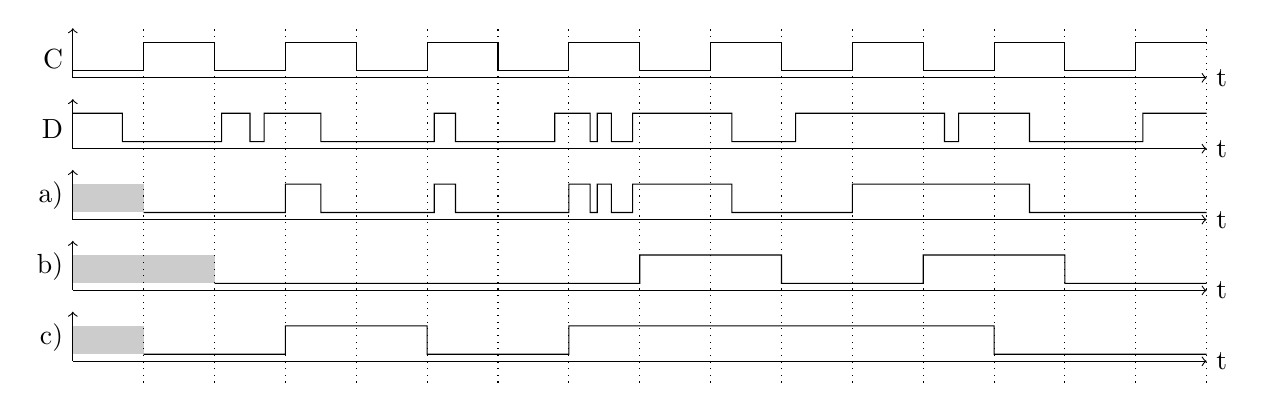
\begin{tikzpicture}[scale=.9]

% helpers
\def\hAzero{2.4}  \def\hAone{2.8}
\def\hBzero{1.4}  \def\hBone{1.8}
\def\hCzero{0.4}  \def\hCone{0.8}
\def\hCyzero{4.4} \def\hCyone{4.8}
\def\hDzero{3.4}  \def\hDone{3.8}

\def\diff{.4}

% undefs
\def\drawundef#1#2{\fill[gray!40] (0, #1) rectangle ++(#2, -\diff);}
\drawundef{\hAone}{1}
\drawundef{\hBone}{2}
\drawundef{\hCone}{1}

% grid
\foreach \name/\y in {C/5,D/4,a)/3,b)/2,c)/1}{
  \draw[<-] (0,\y) -- ++(0,-.7) node[anchor=south east] {\name};
}
\foreach \y in {.3,1.3,2.3,3.3,4.3}{
  \draw[->] (0,\y) -- ++(16,0) node[anchor=west] {t};
}
\foreach \x in {1,...,16}{
  \draw[dotted] (\x, 0) -- ++(0,5);
}

% draw helpers
\def\drawAt#1#2{\draw (#1,#2) -- ++(1,0);}
\def\connect#1#2{\draw (#2,#1) -- ++(0,\diff);}

% draw cycle
\foreach \x in {0,2,...,15}{
  \drawAt{\x}{\hCyzero}
  \connect{\hCyzero}{\x}
}
\foreach \x in {1,3,...,15}{
  \drawAt{\x}{\hCyone}
  \connect{\hCyzero}{\x}
}

% draw D
\def\up{, \hDzero) -- ++(0, \diff) -- (}
\def\dn{, \hDone)  -- ++(0, -\diff) -- (}
\draw (0, \hDone) -- (.7 \dn 2.1 \up 2.5 \dn 2.7 \up 3.5 \dn 5.1 \up 5.4 \dn 
                     6.8 \up 7.3 \dn 7.4 \up 7.6 \dn 7.9 \up 9.3 \dn 10.2 \up
                     12.3 \dn 12.5 \up 13.5 \dn 15.1 \up 16, \hDone);

% draw A
\def\up{, \hAzero) |- ++(0, \diff) -- (}
\def\dn{, \hAone)  -- ++(0, -\diff) -- (}
\draw (1, \hAzero) -- (3 \up 3.5 \dn 5.1 \up 5.4 \dn 7 \up 7.3 \dn 7.4 \up 7.6 \dn 7.9 \up 9.3 \dn 11 \up
 13.5 \dn 16, \hAzero);

% draw B
\def\up{, \hBzero) -- ++(0, \diff) -- (}
\def\dn{, \hBone)  -- ++(0, -\diff) -- (}
\draw (2, \hBzero) -- (8 \up 10 \dn 12 \up 14 \dn 16, \hBzero);

% draw C
\def\up{, \hCzero) -- ++(0, \diff) -- (}
\def\dn{, \hCone)  -- ++(0, -\diff) -- (}
\draw (1, \hCzero) -- (3 \up 5 \dn 7 \up 13 \dn 16, \hCzero);


\end{tikzpicture}
\end{center}



\end{document}
